\documentclass[letter]{article}
\usepackage[english]{babel}

%Inline lists
\usepackage[inline]{enumitem}
%Mention after author's name
\usepackage[affil-it]{authblk}
%Code for adding link to footnote
\usepackage{hyperref}
\newcommand{\footlink}[2]{\href{#1}{#2}\footnote{\url{#1}}}
%Inline code formatting
\usepackage{xcolor}
\usepackage{minted}
\usemintedstyle{manni}
\setmintedinline{breaklines}
\definecolor{linkblue}{HTML}{42a6d4}
\hypersetup{
    colorlinks,
    linkcolor={black},
    citecolor={linkblue},
    urlcolor={linkblue}
}

%Including graphics
\usepackage{graphicx}
%Bibliography
\usepackage[backend=biber,citestyle=authortitle-ibid,bibstyle=ieee,uniquename=init]{biblatex}
\addbibresource{bibliography.bib}
%https://tex.stackexchange.com/questions/151217/remove-parentheses-for-empty-year-field-biblatex-ieee-style#151264
\usepackage{xpatch}
\xpatchbibdriver{online}
  {\printtext[parens]{\usebibmacro{date}}}
  {\iffieldundef{year}
    {}
    {\printtext[parens]{\usebibmacro{date}}}}
  {}
  {\typeout{There was an error patching biblatex-ieee (specifically, ieee.bbx's @online driver)}}
%Spacing between paragraphs
\setlength{\parskip}{\baselineskip}

\title{ActumCrypto Blockchain System}

\author{Ryan Shane}
\affil{Creator/Developer, ActumCrypto}
\author{Ben Schattinger}
\affil{Typesetter}

\date{\today}

\begin{document}
\maketitle

\section{Background}
Security is a major concern among internet users. As they continue to purchase more items online, cryptographically secure digital currencies, or cryptocurrencies, have become more popular. Bitcoin and Ethereum, the two most popular cryptocurrencies have millions of users and thousands of websites, stores, and applications accept their currencies.

As cryptocurrencies have gained support from mainstream financial figures and organizations, their growth has accelerated. A future of digital currencies is very much upon us. A single currency such as Bitcoin, Ethereum, or Ripple, cannot alone replace all other currencies. A single currency with one value becomes impractical when you apply it to multiple sectors. It is practical for investors to have a high valued coin, but practical for the ordinary user to have a low valued one, so they don’t pay everything in fractional amounts.

In addition, cryptocurrencies, while their algorithms are hard to break, are far from perfect in terms of security. Hackers have stolen hundreds of thousands of dollars worth of cryptocurrencies, exchanges have stolen money and shut down and scams have stolen even more. Distrust of these services, along with lack of technical experience, have caused many to be wary of, and avoid these currencies.

Cryptocurrencies run on a decentralized, peer to peer, node based system called a blockchain. In a blockchain, each transaction is stored in blocks, and each node stores a record of every block, and therefore every single transaction on the blockchain. This prevents a hacker from just changing the ledger, because they would have to change a majority of nodes to do so. As of 2018, Bitcoin had 11637 nodes reachable by the Bitnodes crawler\footcite{bitnodes}, and potentially thousands more, making this kind of attack very difficult, if not impossible. The way that an attacker would actually execute this would be to seize 51\% or more of the total hashing power. This is known as a 51\% attack.

\section{Shortcomings of Other Cryptocurrencies}
\subsection{Proof-of-Work and Proof-of-Stake Mining}
Bitcoin is based on Proof-of-Work (PoW) mining. In proof of work mining, each block is only accepted when a computer finds a difficult hash as a “Proof-of-Work”. When a computer winds a difficult enough hash, they broadcast it to all nodes, which verify the block, and only accept it if the transactions are valid and not already spent. This means that the voting for the accepted blockchain register is one-vote-per-CPU.\footcite{bitcoin}

Ethereum uses Proof-of-Stake (PoS) based mining. PoS has a few advantages over PoW, including reduced energy usage, less chance of centralization, and the ability to make 51\% attacks much harder.\footcite{ethereum_proof_of_stake} Proof-of-Stake delegates votes based on the amount of currency the computer has. PoS miners therefore have less incentive to attack, since they would be attacking their own holdings. PoS is not perfect, however. PoS miners have no incentive to agree in the future (also known as a consensus failure), and thus they have “nothing at stake”. Because of this, there is an increased chance of spending currency multiple times during forks or other reorganizations.\footcite{potter_2017}

\subsection{High Energy Usage}
Bitcoin is estimated to use 52.94 TWh of electricity this year,\footcite{digiconomist} or enough to power 4917 homes for a year. This takes a toll on our environment. While there are advances in renewable, fossil fuels are the main source of power for electricity plants, meaning that Bitcoin mining is partially leading to the decline of our environment, and the additional electricity could be used to power more homes or used for other reasons.

The main reason that Bitcoin uses so much electricity is that PoW mining is a global race to solve a mathematical problem, and so large amounts of computing power are required in order to win that race. Thousands of high-end GPUs and other mining devices use large amounts of electricity, leading to far increased consumption of electricity. This also not only takes a toll on the environment, but also on miners profits, as they must pay for electricity, and gamers, who also want the high-end GPUs that are necessary to mine Bitcoin and other PoW cryptocurrencies.

\subsection{Transaction Fees}
Many blockchains charge fees for transactions of their cryptocurrencies. These fees may seem negligible at first, but as many online purchases move to cryptocurrencies, these fees are becoming more relevant. Transaction fees drive potential consumers and merchants away from cryptocurrencies. Because PayPal and credit cards have comparable fees, merchants would rather present customers with familiar options.

The average transaction fee for ethereum is around \$0.76,\footnote{As of March 2018} which may not seem like much, but for a trader making hundreds of trades a second or an online shopper purchasing items online it can make a significant difference. The average online shopper in North America makes 19 purchases a year,\footcite{statista} and so therefore the average shopper would pay \$14.63 in transaction fees at current prices. However, as consumers purchase more and more things using cryptocurrencies and other digital payment methods, transaction fees will be applied to more purchases. Also, since there are no direct charges to the consumer (the merchant is charged instead) through some payment systems, such as PayPal, customers would rather use these systems.

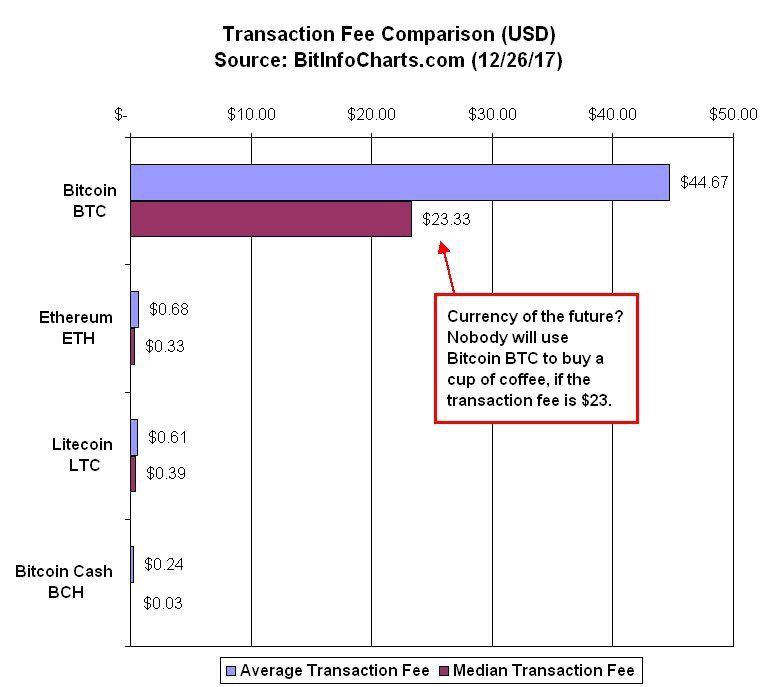
\includegraphics[width=\textwidth]{bitcoin_fees}

Cryptocurrencies are now being used in real world setting, such as buying coffee, food, or other common items. Transaction fees, however, make that much more expensive. Even if the fee is \$0.50 on a cup of coffee, if you buy one cup everyday for a year, you spend \$182.50 unnecessary dollars.

\subsection{Centralization}
Having a central authority can cause slowdowns, bias, and loss of privacy. The main reason to have a blockchain is to avoid these drawbacks of having a central authority. However, many cryptocurrencies have become centralized. These include \begin{enumerate*}[label=(\alph*)]\item Ripple - Validators are decided by the Ripple company, \item NEO - A single party controls the 7 trusted nodes, and \item IOTA - The “coordinator” is a central authority.\end{enumerate*} These are just a few examples, but there are many cryptocurrencies and blockchains that have become centralized, either purposefully, or as a result of one party seizing nodes and mining power. A 51\% attack can not only allow attackers to steal coin, it can also allow them to become a centralized authority.

\section{ActumCrypto}
\subsection{Introduction}
The solution to the shortcomings of many cryptocurrencies is ActumCrypto. ActumCrypto aims to improve upon the models of many cryptocurrencies and overcome the problems of 51\% attacks, high energy usage, centralization, and transaction fees. ActumCrypto is based on Multichain, an open-source system for creating blockchains. ActumCrypto supports Windows, Linux, and Mac users by creating ActumWallet, the “core” wallet for ActumCrypto, and ActumMiner, the “core” mining software for ActumCrypto in Java, allowing ActumCrypto to be cross platform and support all users.

Since transaction fees are a clear detriment to the ease of use of a cryptocurrency, ActumCrypto has zero transaction fees. The only reward for nodes on the ActumCrypto blockchain is from mining. This will allow ActumCrypto tokens to be used for day to day purchases such as coffee, food, clothes, and gas, as well as larger purchases such as cars, and investments. Additionally, because there are no charges to the consumer or merchant, there is an incentive for both to use ActumCrypto over other payment methods. This is especially helpful for merchants who accept credit cards and PayPal, as they are charged for using them, affecting their bottom line.

\subsection{Tokens}
While it may make some sense to have separate currencies, one for investing in, one for general use, one for this, one for that, having so many blockchains means you have to store a lot of data. Tokens, however, are all on the same blockchain and have a couple of key advantages: \begin{enumerate*}[label=(\alph*)]\item less storage space required, \item atomic exchanges within the blockchain, and \item easier switching between currencies.\end{enumerate*}

Less storage space is required for many cryptocurrencies that exist as tokens on one blockchain. This is because there is a certain amount of identifying metadata wrapped around every block, and instead of having that metadata repeated 100 times for 100 currencies, it can be repeated only once. This will help prevent the blockchain from exceeding the capacity of average computers as the transaction throughout increases.

Atomic exchanges are a direct swap of two tokens or cryptocurrencies. Within the ActunCrypto blockchain they are defined by two amounts, one of each of two assets. With an atomic exchange, one wallet would send an amount of one token and the second would send the corresponding amount of another token instantaneously, completing the swap. This type of exchange works well for fast trading, currency exchanges and anything else where swapping currencies is key. Having both currencies as tokens on one blockchain slashes the time needed to proceed the transaction, as no external communication is required. Atomic exchanges on ActumCrypto are achieved using the steps \footlink{https://www.multichain.com/developers/atomic-exchange-transactions/}{here}.


Tokenization is a core principle of ActumCrypto. Within ActumCrypto, all cryptocurencies exist as tokens, including ActumCoin. Because tokenization is so important to ActumCrypto, any developer can create tokens with smart contracts. To create a token, the developer simply must call an issue api call. This is also implemented in \mintinline{java}{TokenManager}, using \mintinline{java}{TokenManager.issue(tok, amount, initialAddress)}. Tokens have ``tok names'' which are three character versions of their name that are used for reference on the blockchain and real names which are the names one would use to discuss them.

\subsection{ActumCoin}
ActumCrypto is a heavily tokenized blockchain, meaning that it embraces the need for having many tokens. However, there is still a need for a native, or default token/cryptocurrency. On ActumCrypto, this is ActumCoin. ActumCoin behaves exactly like every other token on the blockchain, with two special additions. These additions are \begin{enumerate*}[label=(\alph*)]\item all pay-outs/rewards from mining are always in ActumCoin, and \item ActumCoin will be initially created with ActumCrypto.\end{enumerate*} Because there are many tokens on ActumCrypto, all payouts are in the native currency, ActumCoin.

The initial issue amount of ActumCoin, which is tok \texttt{ACM}, is \texttt{15,000}. Of this amount, \texttt{10,000} will be released in the initial offering, with the remainder going to the developer and testers. Upon initial release of ActumCrypto, ActumCoin will be available for \$0.10 each. ActumWallet will be available 10 minutes before the initial offering of ActumCoin, in order to allow users to install and set it up. ActumMiner will be released at the same time as the initial offering.

\subsection{Smart Contracts}
A smart contract is a piece of software programmed to automatically facilitate, verify, or enforce the execution of a contract.\footcite{smart_contract} Smart contracts are programmed such that once both sides agree to a contract, one party cannot cheat, scam, or short the other. These are especially useful in situations where you are sending a traditional currency to an exchange to buy some of a cryptocurrency, or with purchasing digital files, where once the cryptocurrency is received, the files are automatically sent. The source code of smart contracts should also be at least visible and un-obfuscated to both parties, if not open-source, such that both parties can verify that the smart contract will perform the task required and not violate the agreement.

In order to increase protection for consumers, all automated payment systems should use smart contracts. In order to help more developers incorporate smart contracts into their applications, ActumCrypto allows api commands to be called on nodes. These commands include sending tokens, issuing tokens, and retrieving balances. These connections are also protected with a username and password. In addition, in the \footlink{https://github.com/ActumCoin/SmartContracts}{SmartContracts} repository on Github, there are a few example smart contracts in Java. These include the packages \texttt{balance} and \texttt{token} which contain helper classes that allow you to easily call and parse certain api commands on ActumCrypto. Lastly, \footlink{https://github.com/SimplyUb/MultiChainJavaAPI}{\texttt{MultiChainJavaAPI}} also works with ActumCrypto and is the backbone of the balance and token packages.

\subsection{Mining}
ActumCrypto utilizes a semi-round robin form of mining. Using a factor called mining diversity, we are able to distribute the mining power equally. This prevents one miner from monopolizing the mining process. The ActumCrypto blockchain automatically follows these steps every block.
\begin{enumerate}
\item Count the number of miners
\item Multiply that number by mining diversity to get \texttt{spacing}, and round
\item If the miner of this block mined one of the past \texttt{spacing-1} blocks, this block is invalid and another miner must mine it
\end{enumerate}

The mining diversity of ActumCrypto is \texttt{0.625}, a number chosen to distribute the mining power, while making sure that inactive miners don’t cause the blockchain to freeze.

By restricting miners to only 1 block every \texttt{spacing} blocks, it is impossible to have a single miner control the blockchain, unless there is only one miner. However, even if multiple miners work together to attempt to take control, the round robin system requires other miners to eventually take over, thus changing a 51\% attack to have to be a 63\% attack, which requires control of 12\% more of the total miners. If mining diversity was higher, this could potentially be increased until the attack would require 100\% of miners, but since some miners may be inactive, that is not possible without the blockchain freezing.

The high energy usage that is required to power Bitcoin miners and the lower, but still high energy usage for Ethereum miners can be avoided with this style of mining. Since miners cannot mine as much, and the mining is spread out, there are very few benefits from high power and high energy components. This not only is better for the environment, but also has the potential to end the current shortage of graphics cards.

As mentioned before, all rewards from mining a block are in ActumCoin. The reward from mining a block initially will be \texttt{16 ACM}, but the reward will halve every \texttt{524,288} blocks. As an example, the 10th block would reward its miner with \texttt{16 ACM}, while the 1,048,577th would reward them with \texttt{4 ACM}. This is to prevent the extreme hyperinflation of ActumCrypto and keep balances within “reasonable” amounts. Even so, after \texttt{2,097,152} blocks, when the reward is at \texttt{1 ACM}, there will be \texttt{16,262,928 ACM}. The reward will, of course, continue to halve, although, at some point, it may be fixed at its current value.

In order to prevent miners from simply using separate instances of the mining program to circumvent the round-robin system, miners are rewarded for “loyalty”. The more blocks a miner mines, the higher percentage of the reward the receive. This is calculated using the formula $\frac{2}{15}m^{n}$, where `m` is mining diversity and `n` is the number of previous blocks the miner has mined. 
\subsection{Conclusion}
In order to fix many of the shortcomings of popular cryptocurrencies, a new form of blockchain is required. ActumCrypto is a tokenized blockchain with round-robin mining, no transaction fees, and smart contracts, solving these problems. By tokenizing the blockchain, storage space is reduced, and atomic exchanges become easier. Round-robin mining helps reduce energy usage, free up high power components for other work-loads like servers and gaming, and prevent 51\% attacks. Smart contracts help prevent fraud, scams, and make the usage of cryptocurrencies safer and more fair.
\pagebreak

\section{Acknowledgements}
Thanks to Ayham Harb and Ben Schattinger for the helpful feedback.

\section{Revisions}
March 9, 2018, Original

March 14, 2018, Added "loyalty" to Mining section and switched to LaTeX

\newpage
\printbibliography
\end{document}
